\documentclass[12pt]{amsart}
%\documentclass{amsart}
\usepackage[utf8]{inputenc}
\usepackage{graphicx}
\usepackage{amssymb}
\usepackage{amsmath}
\usepackage{epstopdf}
\usepackage{amsthm}
\usepackage{xypic}
\usepackage{enumerate}
%\usepackage{sidenotes}

%\usepackage{fourier}
%\usepackage{a4wide}


\newtheorem{definition}{Definition} 
\newtheorem{proposition}[definition]{Proposition} 
\newtheorem{theorem}[definition]{Theorem} 
\newtheorem{lemma}[definition]{Lemma} 
\newtheorem{corollary}[definition]{Corollary}
\newtheorem{conjecture}[definition]{Conjecture}
\newtheorem{question}[definition]{Question}
\newtheorem{claim}[definition]{Claim}
\newtheorem{fact}[definition]{Fact}
\newtheorem{remark}[definition]{Remark}
\newtheorem{wedgelemma}[definition]{Wedge Lemma} 
\newtheorem{construction}[definition]{Construction}
\newtheorem{example}[definition]{Example}


\newcommand{\lo}{\preceq}
\newcommand{\rar}{\rightarrow}
\newcommand{\rAr}{\Rightarrow}
\newcommand{\lrAr}{\Leftrightarrow}
\newcommand{\RR}{\mathbb{R}}
\newcommand{\NN}{\mathbb{N}}
\newcommand{\QQ}{\mathbb{Q}}
\newcommand{\ZZ}{\mathbb{Z}}
\newcommand{\HHH}{\mathcal{H}}
\newcommand{\AAA}{\mathcal{A}}
\newcommand{\SSS}{\mathcal{S}}
\newcommand{\FFF}{\mathcal{F}}
\newcommand{\K}{\mathbf{K}}
\renewcommand{\L}{\mathbf{L}}
\newcommand{\U}{\mathbf{U}}
\newcommand{\V}{\mathbf{V}}
\newcommand{\X}{\mathbf{X}}
\newcommand{\Rat}{\operatorname{Rat}}
\newcommand{\ehr}{\operatorname{ehr}}
\newcommand{\dist}{\mathsf{dist}}
\newcommand{\sgn}{\mathrm{sgn}}
\newcommand{\sprod}[2]{\langle #1, #2 \rangle}
\newcommand{\mspan}{\operatorname{span}}
\renewcommand{\dim}{\mathsf{dim}\ }
\newcommand{\inter}{\mathsf{int}\ }
\newcommand{\median}{\mathrm{median}\ }
\DeclareMathOperator*{\argmin}{arg\,min}

\newcommand{\defn}[1]{\emph{#1}}
\newcommand{\norm}[1]{|| #1 ||}

\newcommand{\Glat}{G^{\operatorname{lat}}}
\newcommand{\Gdep}{G^{\operatorname{dep}}}
\newcommand{\Gfine}{G^{\operatorname{fine}}}
\newcommand{\Gfinem}{G^{\operatorname{fine*}}}

\newcommand{\FD}{\mathcal{F}}

\newcommand{\path}{\operatorname{path}}
\newcommand{\reldep}[2]{{#1} \longrightarrow {#2}}
\newcommand{\reldepi}[3]{{#1} \overset{#2}{\longrightarrow} {#3}}
\newcommand{\shift}[2]{\rightarrow(#1,{#2})}
\newcommand{\shiftw}[3]{\overset{#1 \cdot #2}{\longrightarrow} {#3}}

\newcommand{\conv}{\operatorname{conv}}
\newcommand{\cone}{\operatorname{cone}}
\newcommand{\lev}{\operatorname{lev}}
\newcommand{\Lev}{\operatorname{Lev}}
\renewcommand{\deg}{\operatorname{deg}}
\renewcommand{\dim}{\operatorname{dim}}
\renewcommand{\min}{\operatorname{min}}
\renewcommand{\max}{\operatorname{max}}
\newcommand{\fract}{\operatorname{frac}}
\newcommand{\integ}{\operatorname{int}}
\newcommand{\relint}{\operatorname{relint}}

\newcommand{\twin}{\mathsf{twin}}
\newcommand{\hull}{\mathsf{hull}}
\newcommand{\diam}{\mathsf{diam}}
\newcommand{\choice}[1]{\left\{ \begin{array}{ll} #1 \end{array} \right.}
\newcommand{\floor}[1]{\lfloor {#1} \rfloor}
\newcommand{\ceil}[1]{\lceil {#1} \rceil}
\newcommand{\mset}[2]{ \left\{ #1 \; \middle| \; #2 \right\}}
\newcommand{\lk}{\mathsf{lk}}
\newcommand{\sd}{\mathsf{sd}}
\newcommand{\Pa}{\mathrm{P}}
\newcommand{\dotcup}{\ensuremath{\mathaccent\cdot\cup}}
\newcommand{\Hom}{\mathrm{ Hom}}
\newcommand{\om}{\omega}

\begin{document}
\title{Scheduling Problems}
\author{Felix Breuer, Caroline J. Klivans}



\begin{abstract}{(Placeholder basically from my talk abstract) We introduce new families of polynomials associated to scheduling problems.  Our starting point is the consideration of counting functions which enumerate the number of solutions to certain scheduling problems.  These scheduling problems arise naturally in the context of the normal fan of a related polytope.  This approach creates a connection to Erhart theory and quasisymmetric functions which allows us to establish polynomiality of the counting functions easily. Moreover, from these perspectives we establish bounds on the coeffiecients of the polynomials, reciprocity theorems and nonnegativity of certain basis exapansions. 

This approach includes certain classic polynomials arising in geometric combinatorics such as the chromatic polynomial, but also polynomials that do not satisfy contraction/deletion and hence are not generally Tutte invariants.  For example, we define the arboricity polynomial which counts the number of matroid covers with a fixed number of independent sets.}
\end{abstract}
\maketitle


\tableofcontents

%%%%%%%%%%%%%%%%%%%%%%%%%%%%%%%%%
\section{Introduction}
%%%%%%%%%%%%%%%%%%%%%%%%%%%%%%%%%



A \defn{scheduling problem} $S$ on $d$ items is given by a boolean formula $\phi$ over atomic formulas $\omega_i\leq \omega_j$ for $i,j\in[d]$. A \defn{$k$-schedule} solving $S$ is a function $\omega:[n]\rightarrow[k]$ such that $\phi(\omega)$ is true.

* Constraint satisfaction problem.



\section{Motivating examples}

*** Illustrate the overall ideas and methods through a motivating example(s).  Choose examples that are not the 'prettiest', namely that would not fall under other methods, and do not just do the chromatic polynomial. ****

Given a graph, most naturally we consider the graphical arrangement,
the subarrangement of the Braid arrangement given by hyperplanes
indexed by edges in the graph.

Given a matroid, we consider the matroid polytope formed by the convex
hull of the support vectors of bases.  The normal fan of the matroid
polytope is refined by the Braid arrangement, but this fan and the
graphical arrangement are not the same.  

We considered the very special case of graphical matroids.  Matroids
whose bases correspond to spanning trees of a graph.  Take the
\emph{matroid polytope} approach to a graphical matroid.  What integer
points / weight classes / relative orderings are induced?  We saw more
complicated 'rules', for example:\\

$x_1 \neq x_2$ if $x_3 \geq x_1$.  But $x_1 = x_2$ is ok if $x_3 < x_1$.\\

We interpreted this as {\bf{scheduling}} of tasks.  Tasks $x_1$ and
$x_2$ can be performed  at the same time only if $x_3$ happens first.

\begin{figure}[h]
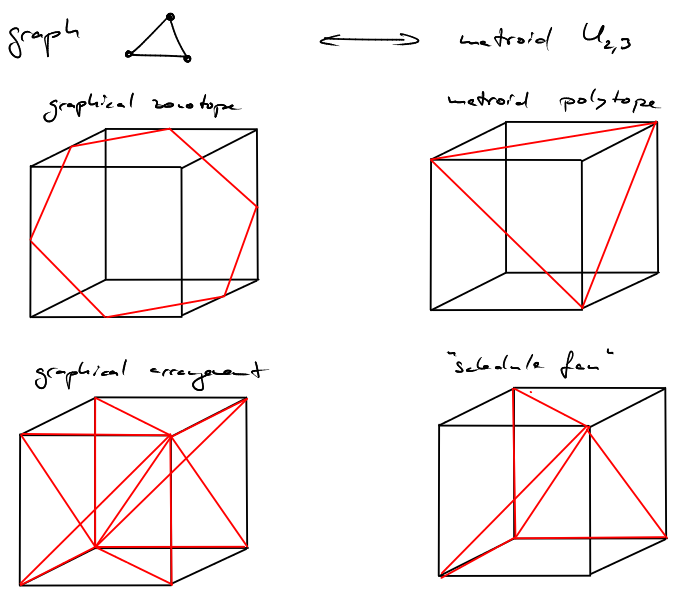
\includegraphics[width=13cm]{graph-matroid}
\caption{Difference between graph construction and graphical matroid construction.}
\end{figure}


\begin{figure}[h]
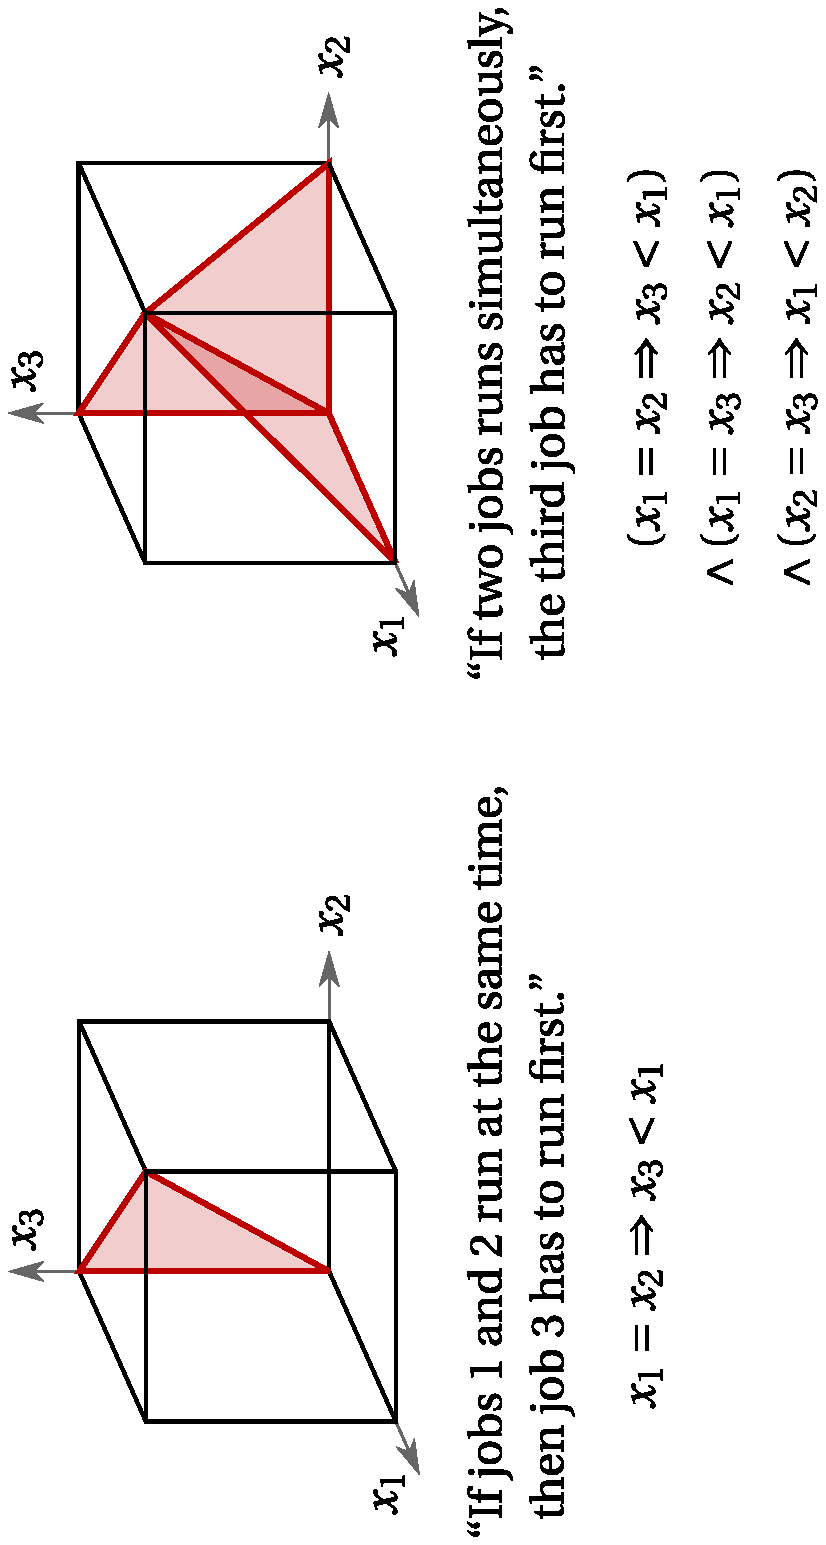
\includegraphics[width=13cm]{schedule}
\caption{Two "scheduling arrangements".}
\end{figure}

One of the staples of geometric methods in combinatorics is to interpret a monomial as an integer point in space. The standard construction is to view a monomial in commuting variables $x_1^{a_1}x_2^{a_2}\cdot\ldots\cdot x_d^{a_d}$ as the point $(a_1,a_2,\ldots,a_d)\in\ZZ^d$. To translate quasisymmetric functions in non-commuting variables into a geometric setting, we need to use a different construction, however. Here we associate to a monomial $x_{i_1} x_{i_2} \cdot \ldots \cdot x_{i_d}$ the point $(i_1,\ldots,i_d)\in \ZZ^d$. For example $x_2x_1x_3$ becomes $(2,1,3)\in\ZZ^3$. That is, the entries of the vector are given by the \emph{indices} of the monomial, as opposed to the exponents. This works because we are working with non-commuting variables here, so that the factors $x_i$ appear in a fixed order.

Quasisymmetric functions in non-commuting variables are going to be introduced in detail in Section~\ref{sec:prelim-qsym}. For now, we just consider the examples in Figure~\ref{fig:cone}. When viewed through the geometric lens explained above the infinite formal sum $\sum_{0<i_3<i_1<i_2} x_{i_1}x_{i_2}x_{i_3}$ in the non-commuting variables $x_1,x_2,x_3,\ldots$, corresponds to the set of integer points $z\in\ZZ^3$ with $0<z_3<z_1<z_2$, that is, the set of integer points in the relative interior of the cone generated by vectors $e_2,e_1+e_2$ and $e_1+e_2+e_3$. If we turn one of the two inequalities into equalities, i.e., we pass to the sums $\sum_{0<i_3<i_1 = i_2} x_{i_1}x_{i_2}x_{i_3}$ and $\sum_{0<i_3=i_1<i_2} x_{i_1}x_{i_2}x_{i_3}$, we obtain two facets of this cone. More precisely, we obtain the set of lattice points in the relative interiors of the cones $\cone_\ZZ(e_1+e_2,e_1+e_2+e_3)$ and $\cone_\ZZ(e_2,e_1+e_2+e_3)$, respectively.

\begin{figure}[h]
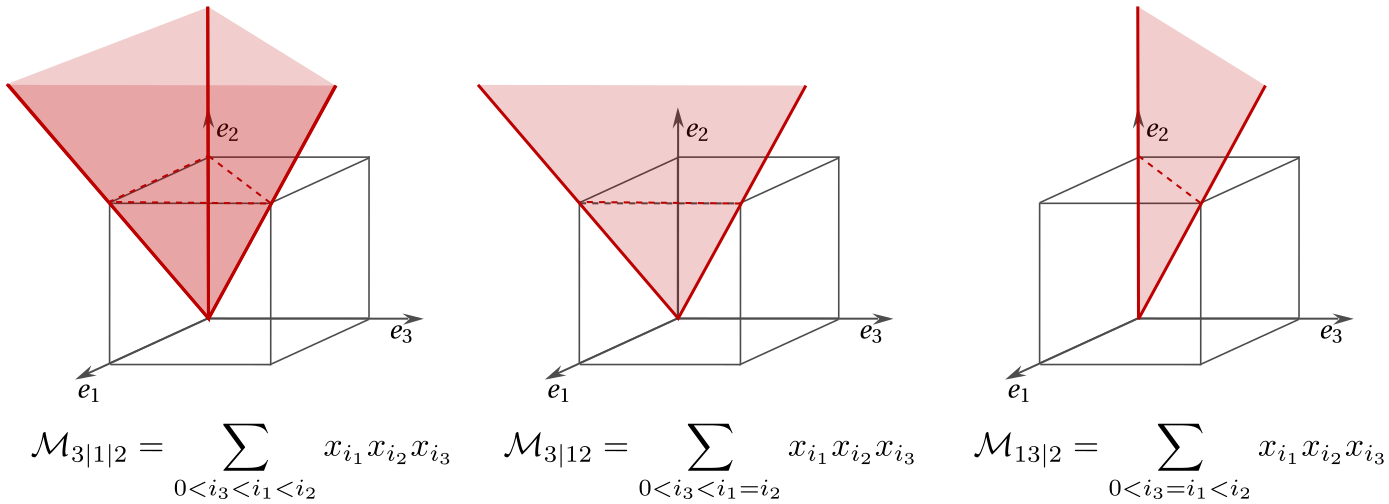
\includegraphics[angle=270,width=14cm]{cone}
\caption{\label{fig:cone}Correspondence between monomial ncquasisymmetric functions and simplicial unimodular cones in the braid arrangement.}
\end{figure}

** In Figure 2, we should replace implies with AND to keep everything a Boolean formula over pairwise comparisions. 

\section{Preliminaries: Ehrhart Theory}

*** cjk: We will need a Preliminaries: Ehrhart Theory section.  I don't know if it should go before or after the next one.
I have given a minimal introduction to the coxeter complex (of type A), quasisymmetric functions and NCQSym.  Telling a very narrow narrative so as to think about these objects specifically the way we want to use them. ***

Consider a (bounded) set $X\subset \RR^d$. The \emph{Ehrhart function} $\ehr_X:\ZZ_{> 0}\rar\ZZ_{\geq 0}$ of $X$ counts the number of integer points in integer dilates of $X$, i.e., \[
  \ehr_X(k) = \#\ZZ^d \cap k\cdot X
\]
for any positive integer $k$. Ehrhart's theorem states that if $X$ is a polytope whose vertices have integer coordinates, then the Ehrhart function $\ehr_X$ of $X$ coincides with a polynomial, called the Ehrhart polynomial of the polytope.

The most important example for our purposes are the Ehrhart polynomials of simplices. The $d$-dimensional \emph{standard simplex} $\Delta^d$ is defined as
\[
  \Delta^d = \mset{x\in\RR^{d+1}}{\sum x_i =1, x_1 \geq 0, \ldots, x_{d+1} \geq 0} = \conv(e_1,\ldots,e_{d+1}).
\]
Its Ehrhart polynomial is given by a binomial coefficient
\[
  \ehr_{\Delta^d}(k) = \binom{k+d}{d} = \frac{1}{d!} (k+d)\cdot (k+d-1) \cdot \ldots \cdot (k+1)
\]
which is a polynomial of degree $d$ in the variable $k$.

There are many other integral simplices which have the same Ehrhart polynomial as the specific ones defined above. An \emph{affine unimodular transformation} is an affine automorphism of the form $x \mapsto Ax + b$ such that $A$ and $b$ are integral and $A$ has determinant $\pm1$. Equivalently, the affine automorphism induces a bijection from $\ZZ^d$ onto $\ZZ^d$. We say that two polytopes $P$ and $Q$ are \emph{lattice equivalent} if there exists an affine unimodular transformation $f$ such that $P=f(Q)$. We define lattice equivalence for polytopes $P\subset \RR^d$ and $Q\subset \RR^{d+l}$ by identifying $\RR^d$ with $\RR^d\times\{0\}^l\subset \RR^{d+l}$. For example, $\Delta^d$ is lattice equivalent\footnote{} to the simplex
\[
  \mset{x\in\RR^{d}}{\sum x_i \leq 1, x_1 \geq 0, \ldots, x_{d} \geq 0} = \conv(0,e_1,\ldots,e_d).
\]  It is straightforward to check that lattice equivalent polytopes have the same Ehrhart polynomial. We will call simplices that are lattice equivalent to a standard simplex \emph{unimodular simplices}. Note that all faces of a unimodular simplex are themselves unimodular.

Ehrhart polynomial of unimodular simplices arise naturally from the study of scheduling problems. Consider the following scheduling problem: "Schedule two jobs, 1 and 2, such that job 2 starts after or at the same time as job 1." Suppose jobs can be run in discrete time slots, numbered $0$ through $k$. A feasible schedule is a pair of integer numbers $0\leq x_1,x_2 \leq k$ such that $x_1 \leq x_2$. The feasible schedules are precisely the integer points $x=(x_1,x_2)$ contained in the $k$-th dilate of the unimodular simplex $\conv(0,e_2,e_1+e_2)$. Therefore, if we let the deadline $k$ vary, the number of feasible schedules is given by the Ehrhart polynomial of a 2-dimensional unimodular simplex, $\ehr_{\Delta^d}(k)=\binom{k+2}{2}$.

What if, instead, we require job 2 to run strictly after job 1? In this case, feasible schedules are integer points $x\in\ZZ^2$ such that $0\leq x_1,x_2 \leq k$ and $x_1 < x_2$. The strict inequality gives rise to a \emph{half-open simplex}: The $d$-dimensional standard simplex $\Delta^d_i$ with $i$ open faces is defined just as standard simplex above, except that $i$ of the inequalities are strict. More precisely
\[
    \Delta^d_i = \mset{x\in\RR^{d+1}}{\sum x_i =1, x_1 \geq 0, \ldots, x_i > 0, x_{i+1} \geq 0, x_{d+1} \geq 0}.
\]
For every face of the standard simplex that we open, we have to shift the Ehrhart polynomial by one:
\[
  \ehr_{\Delta^d_i}(k) = \binom{k+d-i}{d}.
\]
In particular, the open simplex $\Delta^d_{d+1} = \relint{\Delta^d}$ has Ehrhart polynomial $\ehr_{\Delta^d_{d+1}}(k) = \binom{k-1}{d}$. The feasible schedules in the example mentioned above therefore correspond to the integer points in the $k$-th dilate of a $2$-dimensional unimodular simplex with $1$ open face, and their number is $\ehr_{\Delta^2_1} = \binom{k+1}{2}$.

But half-open simplices do not suffice to capture all scheduling problems. Consider the following variation of our running example: "Schedule two jobs, 1 and 2, such that job 2 starts strictly after job 1. However, if job 1 starts immediately, then both can run at the same time." The exception that both jobs may run simultaneously if they are started immediately adds one point to our half-open simplex: the origin $(0,0)$. The resulting set is no longer a half-open simplex. In fact, it is not even the set-theoretic difference of two closed polytopes. In order to capture this type of geometric object, we work with partial polytopal complexes.

A \emph{polytopal complex} $K$ is a finite set of polytopes in some $\RR^d$ such that $K$ is closed under taking faces and the intersection of any two polytopes in $K$ is a face of both. A polytopal complex is \emph{integral} if all vertices have integer coordinates. We define the \emph{relative interior} of a polytope to be the interior of the polytope taken with respect to its affine hull, so that, for example, the interior of a 2-dimensional triangle in 3-space is the triangle minus its edges and vertices. This definition is important because of the following property: The union of all faces of a polytopal complex is equal to the \emph{disjoint} union of the relative interiors of all faces. For example, a triangle is equal to the open 2-dimension region, plus the open line segments corresponding to the edges, plus the vertices (which are open in their 0-dimensional affine hull). This observation implies that the Ehrhart function of a polytopal complex is just the sum of all Ehrhart functions of the relative interiors of all faces.

Now, how about our half-open triangle with that one extra point? It can be written as the disjoint union of the open 2-dimensional region, the open line segments corresponding to the two closed edges, and the two vertices that we want to include: the origin and $e_2$. However, we exclude the open line segment from 0 to $e_1+e_2$ and the vertex $e_1+e_2$ from the union. This idea of taking the relative interiors of just some of the faces of a polytopal complex gives rise to the notion of a \emph{partial polytopal complex}, which can be defined simply as the disjoint union of a finite collection relatively open polytopes. A partial polytopal complex is integral if all vertices\footnote{In this context, the term "vertices" refers to the vertices of the polytopal complex obtained by taking the closure of all faces in the partial polytopal complex.} have integer coordinates. The Ehrhart function of a partial polytopal complex is simply the sum of the Ehrhart functions of the open faces contained in it, and if the complex is integral it is straightforward to show that the Ehrhart function is again a polynomial. In the example of half-open simplex with the extra point, we can thus observe that its Ehrhart function is $\binom{k+1}{2} + 1$.

This motivates the following observation: If $K$ is a partial simplicial complex in which all vertices are integral and all simplices are unimodular. Then, the Ehrhart function $\ehr_K$ satisfies
\[
  \ehr_K(k) = \sum_{i=0}^d f_i^* \binom{k-1}{i}
\]
where $d$ is the dimension of $K$ and $f_i^*$ denotes the number of $i$-dimensional faces in $K$. As it turns out the polynomials $\binom{k+d-i}{d}$ form a basis of the space of polynomials of degree at most $d$. This implies that every Ehrhart polynomial can be written in the above form and the $f_i^*$ are coefficients of the polynomial with respect to this binomial basis.\footnote{A somewhat surprising fact is that the coefficients $f_i^*$ are non-negative integers for every integral partial polytopal complex, even if it \emph{cannot} be triangulated into unimodular simplicies. (Moreover, there is still a counting interpretation for the $f_i^*$ in that case.) However, this case will not concern us here, as all scheduling problems give rise to partial polytopal complexes that do have a unimodular triangulation.} Note that, equivalently, the coefficients $f_i^*$ can be defined through the generating function identity
\[
\sum_{k \geq 0}\ehr_K(k) z^k = \frac{f^*_0 z^1}{(1-z)^1} + \ldots + \frac{f^*_d z^{d+1}}{(1-z)^{d+1}}.
\]

Similarly, if a partial simplicial complex $K$ be partitioned into half-open unimodular simplices $\Delta^d_i$, then the Ehrhart function $\ehr_K$ satisfies
\[
  \ehr_K(k) = \sum_{i=0}^{d+1} h_i^* \binom{k+d-i}{d}
\]
where $h_i^*$ the number of simplices with $i$ open faces in the decomposition. Such partitions are induced, for example, by shellings of simplicial complexes. In the case of a shelling, the above representation is normalized to $h_0^* = 1$. In that case, the coefficient vector is equal to the $h$-vector of the simplicial complex $K$. On the level of generating functions, this identity can be expressed as
\[
  \sum_{k \geq 0} \ehr_K(k) z^k = \frac{\sum_{i=0}^d h_i^* z^i}{(1-z)^{d+1}}.
\]

\section{Preliminaries: Coxeter Complexes, QSym and NCQsym}
\label{sec:prelim-qsym}

\subsection{Quasisymmetric functions}
A quasisymmetric function is a formal power series in infintely many
variables which has bounded degree and is shift invariant.  Namely for
a composition $\alpha$, the coefficients of all terms
$x_{i_1}^{\alpha_1}x_{i_2}^{\alpha_2} \cdots x_{i_k}^{\alpha_k}$,
running over all possible $k$-tuples $\{i_1, i_2, \ldots, i_k \}$, are
the same.


The monomial quasisymmetric function indexed by the composition $\alpha$ is 
$$M_{\alpha} := \sum_{1 \leq i_1 < i_2 < \ldots < i_k}
x_{i_1}^{\alpha_1} \ldots x_{i_k}^{\alpha_k}.$$  One may equivalently
define quasisymmetric functions as any series which may be written as a
linear combination of monomial quasisymmetric functions, i.e. the
monomial quasisymmetric functions form a basis for the ring of all
quasisymmetric functions.  Clearly any collection of
compositions of $n$ gives rise to a quasisymmetric function simply by
taking the sum of monomial quasisymmetric functions indexed by
compositions in the collection.

** cjk: could include here a discuss of quasisymmetric functions that have
been considered in 'geometric combinatorics', chromatic, matroid,
generalized permutahedra **

\subsection{The Coxeter Complex of Type A}
We want to work at the level of ordered set partitions instead of
compositions.  The correct setting is what is known as 
quasisymmetric functions in non-commuting variables, NCQSym.

Before defining these classes, we motivate working with ordered set
partitions by considering the Coxeter complex of type $A$.  Many of
our arguments will be of a geometric nature concerning the structure
of this complex.


An \emph{ordered set partition} or \emph{set composition} $F \vDash
[n]$ is a sequence of sets $(F^1,F^2, \ldots, F^k)$ such that $\forall
i,j$, $ F^i \cap F^j = \empty$ and $\cup_i F^i = [n]$.  The $F^i$ are the
blocks of the ordered set partition and we will often use the notation
$F^1 | F^2 | \ldots | F^k$.  Note that within each block, elements are
not ordered, so the ordered set partition $13|4|2 \vDash [4]$ is the
same as $31|4|2$.

**fb: Are the $F^i$ allowed to be empty?**


The Braid arrangement $\mathcal{B}_n$ is the hyperplane arrangement in
$\mathbb{R}^n$ consisting of hyperplanes $x_i = x_j$ for all $i,j$.
Note that this arrangement is central, that is all hyperplanes contain
the origin, it is also non-essential, that is the collection of
normals to the hyperplanes do not span all of $\mathbb{R}^n$.  The
hyperplanes have a common intersection equal to the line $x_1 = x_2 = \cdots
= x_n$.  Projecting the arrangement to the orthogonal complement of
this line and intersecting with the unit sphere yields a spherical
simplicial complex known as the \emph{Coxeter complex of type $A$}.
It can be realized combinatorially as the baricentric subdivision of the
boundary of the simplex. 

** fb: In the polyhedral geometry setting, this complex
can be obtained as follows: 1) Start with the cube $[0,1]^d$. 2) Triangulate 
this with the braid arrangement. 3) Remove the two vertices consisting of 
only zeros and only ones, and all incident faces. **

** fb: Also, should we mention here that the Coxeter complex is the dual of the face lattice of the permutahedron? **

The faces of the Coxeter complex can naturally be labeled by ordered
set partitions.  Each face of the Coxeter complex is simply a
normalization of a face of the cell decomposition induced by
$\mathcal{B}_n$ on $\mathbb{R}^n$.  A face of the cell decomposition specifies for each pair $i,j$ whether $x_i < x_j$, $x_i > x_j$, or $x_i = x_j$.  Namely, all points in a fixed face have
the same relative ordering of coordinates.  This relative ordering
induces an ordered set partition on $[n]$.  For example, if a face
consists of all points such that $x_{i_1} = x_{i_2} < x_{i_3} =
x_{i_4} = x_{i_5} < x_{i_6}$ then the induced ordered set partition is
$12|345|6$.  Under this correspondence, we see that each facet
corresponds to a partition into blocks of size one (i.e. a full
permutation).  Morover, a face $G_1$ is contained in a face $G_2$ iff
the ordered set partition of $G_1$ coarsens the ordered set partition
corresponding to $G_2$.  Hence a collection of ordered set partitions
closed under coarsening gives a subcomplex of the Coxeter complex.

\begin{figure}
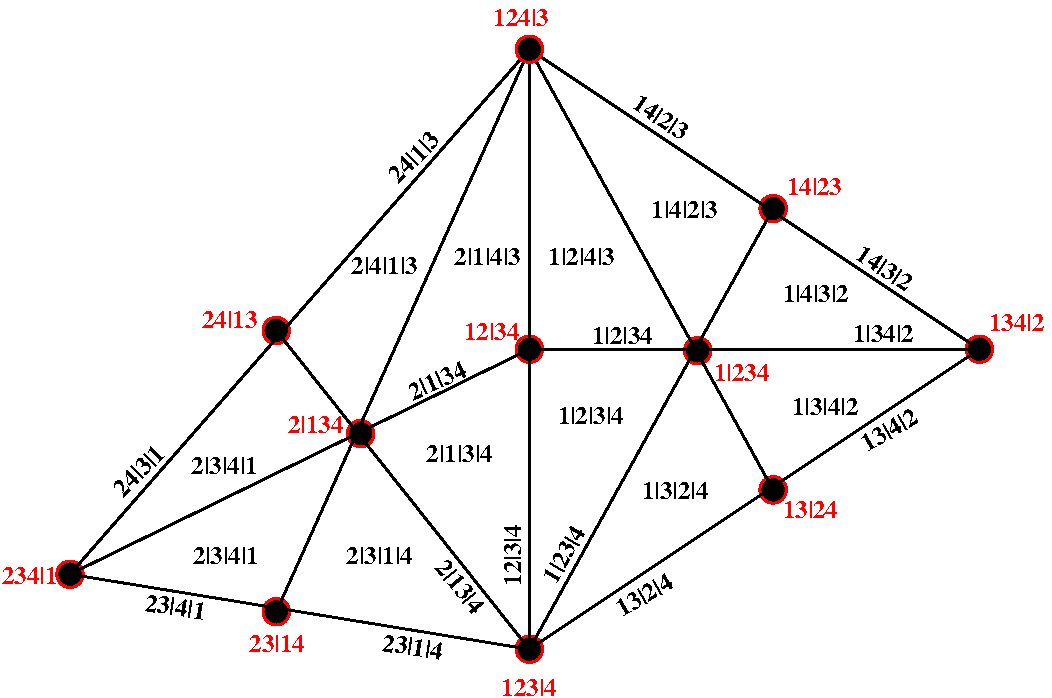
\includegraphics[height=2.5in]{Cox.pdf}
\end{figure}


**Figure of Coxeter complex labeled with ordered set partitions.**

\subsection{Noncommuting Variables}


%% NCSym are symmetric functions indexed by set partitions.  NCQSym are
%% quasisymmetric functions indexed by ordered set partitions, sometimes
%% called set compositions.  (Think of this as analogous to moving from
%% partitions to compositions when one moves from symmetric functions to
%% quasisymmetric functions).


Let $\{x_1, x_2, \ldots \}$ be a collection of non-commuting
variables.  Given $\omega\in \mathbb{R}^n$, let $\mathcal{F}(\omega)$
be the ordered set partition $(F_1,F_2, \ldots F_k)$ such that 
%flag of subsets $\empty = F_0 \subset F_1 \subset \ldots
%\F_{k+1} =[n]$ such that 
$\omega$ is constant on each set $F_i$
%\backslash F_{i-1}$ 
and satisfies $\omega|_{F_i} < \omega|_{F_{i+1}}$ for all $1 \leq i \leq k$. 
%We call $\mathcal{F}(\omega)$ the flag of $\omega$ and
Define the weight class of $\omega$ to be the set of vectors $\nu$
such that $\mathcal{F}(\nu) = \mathcal{F}$.  The weight class $\nu$ consists of all 
points such that the relative size of their components is the same.

\begin{example}
For $\omega = (3,2,2,3,1) \in \mathbb{R}^5$, $\mathcal{F}(\omega) =
(5|23|14)$.  The weight class of $\omega$ consists of all vectors $x
\in \mathbb{R}^5$ such that $x_5 < x_2 = x_3 < x_1 = x_4$. 
\end{example}

Note that
we have again specified the relative ordering of coordinates and a
weight class is simply all points in the relative interior of a cone
of the Braid arrangement and hence naturally associated to a face of
the Coxeter complex.


\begin{definition}
A function in non-commuting variables is called quasisymmetric (an element of NCQsym) if
$\forall \, \gamma, \tau \in \mathbb{N}^n$ such that $\gamma$ and $\tau$
are in the same weight class, $\mathcal{F}(\gamma) =
\mathcal{F}(\tau)$, the coefficient of $x_{\gamma_1}x_{\gamma_2} \cdots
x_{\gamma_n}$ is the same as the coefficient of $x_{\tau_1}x_{\tau_2} \cdots x_{\tau_n}$.
\end{definition}

Let $F$ be an ordered set partition.  Define the monomial quasisymmetric function in non-commuting variables indexed by $F$ as follows:
$$M_F = \sum_{\omega \in \mathbb{N}^n \, \mathcal{F}(\omega) = F} {\bf{x}}_{\omega}$$

Again, one could alternatively define the quasisymmetric functions in
non-commuting variables to be any sum of the monomials.  Most of the
algebra of NCQSym is done at the level of monomials or other bases
indexed by ordered set partitions without reference to the specific
variables.  


\begin{example}

Consider the weight class of  points that satisfy $\omega_1 = \omega_3 < \omega_2 = \omega_4$.  The corresponding ordered set partition $S$ is $(13|24)$.  
$$M_S = x_1x_2x_1x_2 + x_1x_3x_1x_3 + x_2x_3x_2x_3 + x_3x_4x_3x_4 + \cdots$$  

\end{example}

\subsection{From NCQsym to QSym}

As we have seen, elements of QSym are naturally indexed by
compositions and elements of NCQSym are naturally indexed by ordered
set partitions.  We can use the type map from partitions to
compositions to specialize an element of NCQSym to an element of QSym.
The type map of a partition simply records the size of each block.
$$\textrm{type}(B_1|B_2|\cdots|B_n) = (|B_1|, |B_2|, \cdots, |B_n|)$$
If $\mathcal{S} \in NCQSym$ is written as a sum of monomial terms,
applying the type map to each index is equivalent to allowing the
variables to commute.

\begin{example}
Let $\mathcal{S} = M_{(1|23)} + M_{(3|21)} + M_{(2|1|3)}$ be an element of NCQSym written in terms of monomials.  Then 
{type} $\mathcal{S} :=  M_{\textrm{type} (1|23)} + M_{\textrm{type} (3|12)} + M_{\textrm{type} (2|1|3)} = 2 M_{(1,2)} + M_{(1,1,1)}$. Where the right hand side is a quasisymmetric function given in the monomial basis indexed by compositions.  
\end{example}



Given a quasisymmetric function in non-commuting variables (or
commuting), there is also a naturally associated polynomial function
defined by setting the first $m$ variables equal to $1$. 

\begin{example}
Writing ${\bf 1}^m$ for the vector of $1$s of length $m$, and continuing the example above, we have 
$$ \mathcal{S}({\bf 1}^m) = 2 {m \choose 2} + {m \choose 3}$$.  

\end{example}


\section{Scheduling Problems}

Now we have both preliminary sections and should return to scheduling problems.

Define, interpret in both contexts, general theorems.  

*** We also haven't yet talked about hyperplane/polytope duality, generalized permutahedrons, normal fans, the connection to the Braid arrangement.  We can start this section with that material or some of the more general polytope theory can be back in the Erhart section.  For those who would skip a general Erhart section, this is a better place for the material.  It also might make it easier to lead into the technical results.  *****




A \defn{scheduling problem} $S$ on $d$ items is given by a boolean formula $\phi$ over atomic formulas $\omega_i\leq \omega_j$ for $i,j\in[d]$.
 A \defn{$k$-schedule} solving $S$ is a function $\omega:[n]\rightarrow[k]$ such that $\phi(\omega)$ is true. Note that equivalently $\omega$ can also be viewed as a vector $\omega\in [k]^{[n]}$ or as an ordered set partition $\FFF(\omega)$ of $[n]$ into $k$ possibly empty parts. Therefore we will write $\phi(F)$ to mean $\phi(\omega)$ for any $\omega$ such that $\FFF(\omega)=F$ and not that the value of $\phi(F)$ will only depend on $F$ not on the choice of $\omega$. The schedule function $\SSS_S$ in non-commuting variables $x_i$ for $i\in \NN$ is defined as
\[
  \SSS_S = \sum_{\omega\in \NN^n: \phi(\omega) } x_\omega
\] 
The schedule counting function $\xi_S(k)$ is defined as
\[
  \xi_S(k) = \# \text{$k$-schedules $\omega$ such that $\phi(\omega)$ }.
\]


So, geometrically, a satisfiable Scheduling problem can be thought of
as a collection of (relative interiors) of faces of the Coxeter
complex (more correctly, the cell decomposition of space induced by
the Braid arrangement).  This does feel awfully restrictive, it does
not include flow and tension for example as they need (among other
things) the coordinate hyperplanes.  On the other hand, this is a
natural class and perhaps managable for us to make somebroader
statements.



\begin{theorem}
For any scheduling problem $S$ the function $\SSS_S$ in non-commuting variables is a quasisymmetric function of the form
\[
  \SSS_S = \sum_{F: \phi(F)} M_F.
\]

$\SSS_S$ specializes to $\xi_S(k)$ when we substitute $1$ for $k$-different variables in $\SSS_S$ and $0$ for all others. In particular, the result of this specialization is independent of which variables are set to 1. Moreover
\[
  \xi_S(k) = \sum_{i=0}^n f_i^* \binom{k-1}{i}
\]
where $f_i^*$ equals the number of ordered set partitions $F$ of $[n]$ into $i$ non-empty parts such that $\phi(F)$ holds. In particular, the $f_i^*$ are non-negative integers bounded above by $i!\cdot S(n,i)$ where $S(n,i)$ denotes the Stirling numbers of the second kind.

Conversely, for any vector $f=(f_0^*,\ldots,f_n^*)$ of integers between $0$ and $i!\cdot S(n,i)$ there exists a scheduling problems $S$ such that $\xi_S$ has the coefficient vector $f$ with respect to the binomial basis $\binom{k-1}{i}$.
\end{theorem}

There are a couple of other things we could add here:
\begin{enumerate}
\item Add the quasisymmetric function in commuting variables as an intermediate step.
\item $\xi_S$ includes the chromatic polynomial of a graph and the "unknown" matroid polynomial as special cases.
\item $\xi_S$ includes Ehrhart polynomials of order polytopes as a special case.
\item The values of $\xi_S(-k)$ at negative integers can be written as a difference of two counting functions. (This gives "one half" of a reciprocity theorem.) This should also be true on the quasisymmetric function level.
\end{enumerate}

The braid arrangement defines a polyhedral subdivision of the space $\RR^n$, a polyhedral subdivision of the positive orthand $\RR_{\geq 0}^n$ and a polytopal subdivision of the cube $[0,1]^n$. With respect to each of these, we define the \emph{forbidden subcomplex} $\Delta(S)$ to be the set of those faces $\sigma$ of the subdivision such that $\phi(\omega)$ does not hold for any $\omega$ in the relative interior of $\sigma$. Depending on the topological and geometric properties of $\Delta(S)$, we can make various assertions about $\SSS$ and $\xi$. We say $\Delta(S)$ has a convex ear decomposition, if $\Delta(S)$ (viewed as subcomplex of the cube) together with the boundary of the cube, has a convex ear decomposition.

** fb: I think this is almost the same thing as saying that $S$ comes from a generalized permutahedron. It is a tiny bit more general, as this allows regions of the arrangement (i.e. the complement of $\Delta(S)$) to be non-convex. But because the Braid arrangement is so simple, there should be an easier way to define this notion, without referring to convex ear decompositions. **

***cjk: I'm not sure precisely what you mean by $S$ comes from a generalized permutahedron? ***

**** fb: I guess I was trying to say the following. Consider two constructions: 1) Start with a generalized permutahedron and take its face fan. 2) Start with the full permutahedron, take its face fan (which is a polyhedral subdivision of space) and take any subcomplex. 2) is a bit more general than 1) because it allows non-convex regions. ****

\begin{theorem}
Suppose $\Delta(S)$ is simply a valid subcomplex of the Coxeter complex.  Equivalently, the collection of $\omega$ 
corresponding to faces in $\Delta(S)$ are closed under coarsening. (** fb: actually, this should work even for partial polytopal complexes, i.e., $\Delta(S)$ does not need to be closed under coarsening. **) Then:
\begin{enumerate}
\item If $\SSS_S = \sum h_F' L_F$, then the $h_F'$ are non-negative integers.
\item $ \sum_{n \geq 0} ((n+1)^d - \xi_S(n+1)) t^n = \frac{h_{\Delta(S)}(t)}{(1-t)^d} $ \\
(** I worked this out with Marcelo, that paper is not written, may never be, but the credit should go to a preprint**) 
\end{enumerate}
\end{theorem}

\begin{theorem}
Let $S$ be a scheduling problem such that the regions of $[0,1]^n\setminus\Delta(S)$ are the interiors of convex polytopes of dimension $n$. Equivalently, we assume $S$ can be written as a disjunction of conjunctions of strict inequalities, i.e.,
\[
  S = \bigvee_i C_i \text{ where } C_i = \bigwedge_j I_{i,j}
\] 
such that the $I_{i,j}$ are strict inequalities of the form $x_a < x_b$ for some $a$ and $b$, and the conjunctions $C_i$ are satisfiable for all $i$. Then both $\SSS_S$ and $\xi_S$ satisfy a reciprocity theorem:
\begin{enumerate}
\item $\xi_S(-k) = (-1)^n\cdot \#\mset{(i,x)}{S(x) \text{ and } C_i(x)}$
\item TODO: reciprocity for $\SSS_S$.
\end{enumerate}
\end{theorem}

** fb: I'd like to extend the above to include non-convex regions. **

\begin{theorem}
Let $S$ be a scheduling problem such that $\Delta(S)$ is of codimension 1 and has a convex ear decomposition. Then 
\[
  \sum_{n \geq 0} ((n+1)^d - \xi_S(n+1)) t^n = \frac{h_{\Delta(S)}(t)}{(1-t)^d},
\]
as above, and moreover the coefficients $h_i$ satisfy
\begin{enumerate}
\item $h_0 \leq h_1 \leq \ldots \leq h_{\floor{d/2}}$,
\item $h_i\leq h_{d-i}$ for $i\leq d/2$,
\item $(h_0,h_1-h_0,h_2-h_1,\ldots,h_{\ceil{d/2}}-h_{\ceil{d/2}-1})$ is an $M$-vector.
\end{enumerate}
\end{theorem}

A couple of additional points:
\begin{enumerate} 
\item This case still includes chromatic polynomials and the matroid polynomials.
\item Do the convex ear decompositions also tell us something about coefficients on the quasisymmetric function level?
\item Which schedules come from matroids? 
\item Give a simpler sufficient criterion for when there is a convex ear decomposition. For example: There is a convex ear decomposition, if there is a shelling of the Coxeter complex (equiv. the Braid triangulation of the cube) such that the regions of $[0,1]^n\setminus\Delta(S)$ appear consecutively in the shelling.
\end{enumerate}


\begin{enumerate}
\item Section 6 from Tricia and Ed's paper.  They have the wrong polynomial.  Otherwise, all of their results would apply.
\item Other families of polynomials besides Arboricity?  Even known ones that we can simply put into our framework?
\end{enumerate}


A \defn{scheduling problem} $S$ on $d$ items is given by a boolean
formula $\phi$ over atomic formulas $x_i\leq x_j$ for $i,j\in[d]$. A
\defn{$k$-schedule} solving $S$ is a function $x:[d]\rightarrow[k]$
such that $\phi(x)$ is true. The schedule function $\xi_S(k)$ counts
the number of $k$-schedules of $S$.



\subsection{Quasisymmetric functions}

Some ``bigger picture'' thoughts about quasisymmetric functions and a few classes thought about together. 

Consider the following quasisymmetric functions:

\begin{itemize}
\item QGP: (Quasi Generalized Permutahedron) - this includes Stanley chromatic quasisymmetric function for graphs and the Biller-Jia-Reiner quasisymmetric functions for matroids as special cases.

In terms of ordered set partitions, these are all integer points in the interiors of all maximal cones of the fan.  In terms of the forbidden subcomplex, we are getting rid of all codimension one faces.  

\item QBergman: This is defined for any matroid, over the matroid polytope.

\item QEhrenborg: Not really it's name, but Richard defined a class of quasisymmetric functions for posets.

\end{itemize}

\subsubsection{QBergman}

In this section we explore a new instance of a Coxeter quasisymmetric
function, the Bergman quasisymmetric function of a matroid.

Let $M$ be a matroid on ground set $[n]$ and let $\omega \in \mathbb{N}^n$.
We consider $\omega$ to be a weight function on the ground set of $M$ and define the weight of a basis $B$ to be: $\omega(B) = \sum_{e\in B} \omega(e)$. 
%Call a weight function
% $\omega$ on the ground set of a matroid $M$
Furthermore define $M_{\omega}$ to be the induced matroid of all
$\omega$-minimal bases.  Three different perspectives on this induced
matroid are discussed in [ref Section 2].

  We will call $\omega$
$M$-loopless if the matroid $M_{\omega}$ has no loops.  Namely, every
element of the ground set is contained in some minimal weight basis.
(In [ref], such $\omega$ are called {\em valid} and precisely
constitute the integral points of the Bergman fan of $M$.)

\begin{definition}
The Bergman quasisymmetric function is the generating function,
$$QB(M,{\bf x}) := \sum_{M\textrm{-loopless} \, \omega} {\bf x}_{\omega},$$

where ${\bf x}_{\omega} = \prod_{e \in E} x_{\omega(e)}$.
\end{definition}

The fact that $QB(M,{\bf x})$ is in fact a quasisymmetric function follows
from the fact that $M_{\omega}$ is completely determined by the
relative ordering of the componants of $\omega$ and not their exact
value, see [ref Proposition 1].

\begin{example}
$$QB(U_{2,4})  = M_4 + 4M_{1,3}$$

Let us consider what these terms reflect.  The term $4M_{1,3}$
appearing in $QB(U_{2,4})$ reflects the fact that there are $4$
different types of $M$-loopless weight vectors with the form
$\omega_{i_1} < \omega_{i_2} = \omega_{i_3} = \omega_{i_4}$.
(** I am copying an pasting from other notes, so this is written as a quasisymmetric function.  For us, it should be written out as an ncqsym.**)
\end{example}


Again because the weight vector only depends on the relative ordering
of elements, we can correspond a weight vector $\om$ to a flag of
elements in $M$.  Given $\om$, let $\mathcal{F}(\om)$ be the flag 
$$\emptyset =: F_0 \subset F_1 \subset \ldots \subset F_k := [n]$$
where $\om$ is constant on each set $F_i - F_{i-1}$ and $\om|_{F_i - F_{i-1}} < \om|_{F_{i+1} - F_{i}} $.  For example, the weight vector above,  $\om_{i_1} < \om_{i_2} = \om_{i_3} = \om_{i_4}$, corresponds to the flag ${\emptyset \subset \{i_1\} \subset \{i_1,i_2,i_3,i_4\}}$.

\begin{theorem}[Theorem 1 ref]
A weight function $\omega$ is $M$-loopless if and only if it corresponds 
to a flag of flats of $M$.
\end{theorem}


**** {\bf What I want to notice here is that the ordered set partitions I
am picking up for the Quasisymmetric function are closed under
coarsening.  The forbidden subcomplex is an order filter in the
Coxeter complex.  

This quasisymmetric function is not positive in the fundamental (L) basis.  }

Recall that the fundamental basis is defined as:

$$ L_{\alpha} := \sum_{\beta : \beta \, \textrm{refines} \, \alpha} M_{\beta}.$$


Define instead the co-fundamental basis:

$$ N_{\alpha} := \sum_{\beta : \beta \, \textrm{coarsens} \, \alpha} M_{\beta}.$$


Let $f_{\beta} = [M_{\beta}]$ the coefficient of $M_{\beta}$ in
$QB(M)$ in the monomial basis.  Define: 
$$\eta_{\alpha} := \sum_{\beta \leq \alpha} (-1)^{l(\beta)-l(\alpha)}f_{\beta}.$$
Then $\eta_{\alpha} = [N_{\alpha}]$ the coefficient of $N_{\alpha}$ in $QB(M)$ in the cofundamental basis.

\begin{itemize}

\item $\sum_{\alpha} [N_{\alpha}] = 1$ (Alternating sum over subsets)

\item The coefficients $(f_{\beta_1}f_{\beta_2} \dots f_{\beta_n})$ are
a colored refinement of the $f$-vector of the order complex of the
lattice of flats. Flats of the same size (NOT RANK) are given the same
color.

\item If we were working over rank instead of size, we would have the Ehrenborg quasi-symmetric function which runs over flags of flats indexed by rank (as in the lattice).

\item The $\eta$s are a colored refinement of a ``co-h'' vector of the
order complex.  The ``co-h'' is computed via Stanley's trick with the
$f$-vector written backwards from the top down the right hand side and
$f_n$ down the left hand side.

\item $\eta_{|E|} = [N_{|E|}]$ = (sign) Mobius function of the lattice
of flats = (sign) Reduced Euler characteristic of order complex of
proper part of lattice of flats. (It is the alternating sum of the
f-vector just broken up by the refinement).

\end{itemize}



\begin{proposition}
$$[N_{\alpha}] = (-1)^{|\alpha|} \sum_{\alpha \, \textrm{flags}} \prod_i \mu(f_i,f_{i+1})$$
where an $\alpha$-flag is a flag of flats such that $|f_{i+1}| - |f_i| = \alpha_i$ and $\mu$ is the M\"{o}bius function of the lattice of flats of $M$.
\end{proposition}

\begin{corollary}
The sign of $[N_{\alpha}]$ alternates with the length of $\alpha$.  

\end{corollary}



\subsubsection{QEhrenborg}

Ehrenborgs quasisymmetric function gives rise to a quasisymmetric function via ranks (i.e. not the type map, which uses sizes of the pieces).  Given an ordered set partition, interpret it as a flag (in a graded poset) and record the rank jumps of the flag.  

I have put the paper in the dropbox folder: Ehrenborg-Hopf.pdf  

It might be hard to recognize, but see proposition 5.1 which is really the same as the proposition above interpreted via the antipode formula for a Hopf algebra. 

This set-up also gives us ordered set paritions closed under coarsening and hence an order filter in the Coxeter complex. 

But being closed under coarsening is not enough to gaurentee the coefficients result.  The proof in Ehrenborg works for any collection that can be seen as all flags of a graded poset.  I don't know how much further this can be pushed...  


Summary...

\begin{itemize}

\item QBergman and QEhrenborg alternate sign in the co-L basis.  (Closed under coarsening)

\item QGP (inclduing Chromatic and Biller-Jia-Reiner) are positive in the L-basis.  (Closed under refinement)

\end{itemize}

In the second class, it is easy to see geometrically which cones (faces) are being forbidden.  In the first class, it is not easy to see which faces you are taking.  

I haven't spent much time thinking about what the polynomial restrictions of these mean.  

\section{Arboricity}

***cjk: Little intro here that we have seen some known examples of
polynomials that fit into our framework.  Here we demonstrate a new polynomial 
that falls naturally out of our framework. ***


Given a simple graph $G$, the arboricity of $G$ is defined to be the
minimum number of forests needed to decompose (cover) the edges of
$G$.  The parameter was introduced by Nash-Williams and Tutte [refs].
This definition is easily extend to an arbitrary matroid $M$ where the
arboricity becomes the minimum number of independent sets needed to
cover the ground set of $M$.  The constructive version of partitioning
a matroid into as few independent subsetes as possible is known as the
matroid partitioning problem. [History?  Edmonds has first algorithm
  but did he first extend definition to matroids?]  The initial
literature is concerned with computing this minimum number.  As
[Nash-Williams, Tutte, Edmonds] show, the arboricity $a(M)$ is given
by:

$$ a(M) = \textrm{ max}_{X\subseteq E} \lceil { \frac{|X|}{rk(X)}} \rceil . $$

Here we will be concerned with the problem of enumerating independent
set covers by size.  In particular we will show that the number of
covers of $M$ with at most $k$ independent sets is a polynomial in
$k$.  An appropriate analogy to keep in mind is the chromatic
polynomial of a graph.  The chromatic polynomial is the enumerate
function which counts the number of proper coloring of a graph with at
most $k$ colors.  After defining the enumerative function, the first
result one proves is that it is in fact a polynomial function in $k$.
The standard proof follows by induction after establishing a deletion
/ contraction recurrence for the number of colorings.  An important
distinction for counting independent coverings is that they do not
satisfy deletion/contraction hence this standard proof technique will
not apply in our case.  We consider it a particularly appealing aspect
of our theory that the polynomiality of this function follows almost
immediately once the counting function is viewed in our geometric
framework.

\subsection{The Arboricity polynomial}

\begin{definition} Given a matroid $M$ on a finite ground sets $E$, define an independent cover of $M$ with at most $k$ parts to be a mapping $f : E \rightarrow [k]$ such that $f^{-1}(i)$ is an independent set for all $i$.  

  The arboricity polynomial $A_M(k)$ is the counting function equal to the number of independent covers of $E$ with at most $k$ parts.
\end{definition}

**Write out as a  Scheduling problem**

\begin{example}

Let $M$ be the free matroid on a ground set of size $n$; i.e. all subsets of the ground set are independent.  Then $A_M(k) = k^n$.  

\end{example}

\begin{example}

Let $M(C_n)$ be the graphical matroid of the cycle graph on $n$
vertices.  Independent sets of this matroid correspond to acyclic
subsets of edges (forests) of the graph.  For $k \leq 1$ we find no
indpendent covers of $M$.  For $k \geq 2$, indpendent covers
correspond to labeled partitions of $[n]$ with at least $2$ parts.

$$A_{M(C_n)}(k) = \sum_{m=2}^{n} S(n,m) k(k-1) \cdots (k-m+1) $$

Using the identity that $\sum_0^n S(n,m) k(k-1) \cdots (k-m+1) = k^n$, we find:

$$A_{M(C_n)}(k) = k^n - k $$

\end{example}



\begin{example}
Let $M$ be the graphical matroid of the graph $G$ with $5$ edges as
shown in Figure 1.  The entire ground set is not independent so there
are no independent covers of size $1$.  We can achieve independent
partitions of size $2$.  Written as ordered set partitions, they are:
$$ 34e|12, 12e|34, 124|3e, 134|2e, 234|1e, 123|4e, 13e|24, 13|24e, $$
and all those with the order of the blocks reversed, $A_M(2) = 16$.  

Again, in each of the partitions above, within each block of the
partition, the edges form a forest.  These are the partitions of
minimal size, clearly any refinement of these partitions will also
yield independent partitions.

\end{example}

We can utlize this example to show explicitly that $A_M(k)$ does not
satisfy deletion/contraction.  Consider the deletion and contraction
of the edge $e$, $M-e$ and $M/e$.  The independent covers of size $2$
of $M-e$ are
$$ 123|4, 124|3, 134|2, 234|1, 12|34, 13|24, 14|23, $$ and all those
with the order of the blocks reversed.  We could also note that $M-e$
corresponds to a cycle graph and $2^4 - 2 = 14$.  The independent
covers of $M/e$ are $$12|34, 13|24,$$ and those with the order of the
blocks reversed.  Therefore $A_M(2) \neq A_{M-e}(2) + A_{M/e}(2)$.




%\subsection{Quasisymmetric Functions}

%I am assuming that we'll have this general theory set up earlier so I can just work through it in an example. 


****cjk: I just wrote out examples but here we should explicitly describe arboricity in terms of the Erhart and Quasisymmetric picture.  I want to wait to do this until the other sections are written so we can point out specific results that apply.  Also, I actually don't like how all the examples are italized.****


\begin{example}

Consider the matroid of the $3$-cycle $M(C_3)$.  The only circuit is the entire ground set $\{1,2,3\}$.  All other ordered set partitions correspond to independent coverings of $C_3$: 
$$1|23, 2|13, 3|12, 1|2|3,$$
and all those with the order of the blocks permuted. 

Consider the Braid arrangement in $R^3$, the ground set space of the
matroid, or edge set space of the graph.  These ordered set partitions
correspond to the collection of integer points which lie off of the
intersection: $x_1 = x_2 = x_3$.


 Hence the corresponding element of NCQSym is 

$${\bf{{\mathcal A}}}(M) = M_{(1|23)} + M_{(2|13)} + M_{(3|12)} + M_{(23|1)} + M_{(13|2)} +  M_{(12|3)} + $$ $$ M_{(1|2|3)} + M_{(1|3|2)}
+ M_{(2|1|3)} + M_{(2|3|1)} + M_{(3|1|2)} + M_{(3|2|1)}. $$

\noindent Specializing under the type map we have an element of Qsym:

$${\mathcal A}(M) = 3 M_{(1,2)} + 3 M_{(2,1)} + 6 M_{(1,1,1)}. $$

\noindent Evaluating at ${\bf 1}^k $ we have the arboricity polynomial:

$$ A(M) = 3 { k \choose 2} + 3 { k \choose 2} + 6 { k \choose 3} = k^3 - k $$

\end{example}



 \bibliographystyle{amsplain}

 \bibliography{references}

\end{document}
